\documentclass{report}
\usepackage{amsmath}
\usepackage{txfonts}
\usepackage{amsfonts}
\usepackage{amssymb}
\usepackage{mathtools}
\usepackage{geometry}
\usepackage{color}
\usepackage{parskip}
\setlength{\parskip}{1em}
\usepackage{tikz}
\usetikzlibrary{fadings}
\usetikzlibrary{patterns}
\usetikzlibrary{shadows.blur}
\usetikzlibrary{shapes}
\usepackage{multirow}
\newcommand\parrow[3][3ex]{%
 \begin{array}[t]{@{}c@{}} #2 \\
  \left\uparrow\vcenter{\hrule height #1}\right.\kern-\nulldelimiterspace\\
  \makebox[0pt]{\small#3}
  \end{array}%
}
\newcommand\parrowlong[3][6ex]{%
 \begin{array}[t]{@{}c@{}} #2 \\
  \left\uparrow\vcenter{\hrule height #1}\right.\kern-\nulldelimiterspace\\
  \makebox[0pt]{\small#3}
  \end{array}%
}

\geometry{a4paper, margin=1in}

\begin{document}

\setcounter{chapter}{2}

\chapter{Inner Product Spaces}

For a Vector Space over real numbers, an inner product $\langle\cdot \mid \cdot\rangle$ satisfies:

$$
\begin{aligned}
& \langle X \mid Y\rangle=\langle Y \mid X\rangle \\
& \langle X \mid \alpha Y\rangle=\alpha\langle X \mid Y\rangle \\
& \langle X \mid Y+Z\rangle=\langle X \mid Y\rangle+\langle X \mid Z\rangle\\
& \langle X \mid X\rangle \geqslant 0 \text {, and }=0 \text { if and only if } X=0
\end{aligned}
$$

Eg. $\mathbb{C}^{2},\mathbb{C}^{3} \ \langle X \mid Y\rangle=\|X\|\|Y\| \cos (X, Y)$

$  X,Y \in \mathbb{R}^{3}: \ \langle X \mid Y\rangle=x_{1} y_{1}+x_{2} y_{2}+x_{3} y_{3}$ The dot product is $\parrow{an}{But not unique}$ inner product of vectors

Can be extended to $\mathbb{R}^{n}$.

Eg. Integrable functions for $a \leqslant x \leqslant b$.

\begin{center}
    

\tikzset{every picture/.style={line width=0.75pt}} %set default line width to 0.75pt        

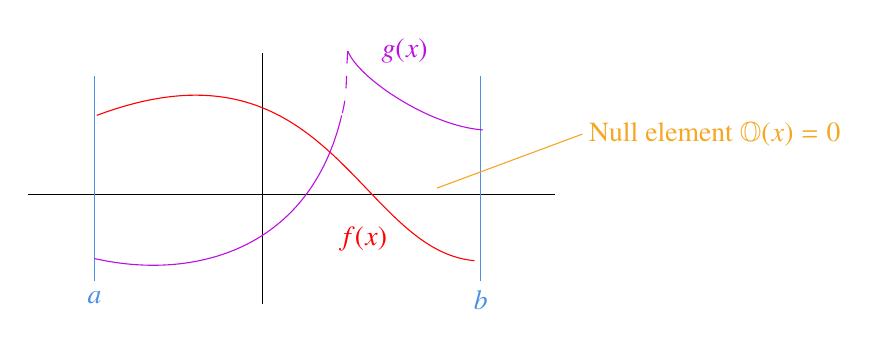
\begin{tikzpicture}[x=0.75pt,y=0.75pt,yscale=-1,xscale=1]
%uncomment if require: \path (0,300); %set diagram left start at 0, and has height of 300

%Straight Lines [id:da28902997561163524] 
\draw    (65,123) -- (319,123) ;
%Straight Lines [id:da33478321711056114] 
\draw    (178,176) -- (178,55) ;
%Curve Lines [id:da28346474586323334] 
\draw [color={rgb, 255:red, 255; green, 0; blue, 0 }  ,draw opacity=1 ]   (98,85) .. controls (210,43) and (224,150) .. (280,155) ;
%Straight Lines [id:da22459181685384633] 
\draw [color={rgb, 255:red, 74; green, 144; blue, 226 }  ,draw opacity=1 ]   (97,165) -- (97,66) ;
%Straight Lines [id:da16540063730298127] 
\draw [color={rgb, 255:red, 74; green, 144; blue, 226 }  ,draw opacity=1 ]   (283,165) -- (283,66) ;
%Curve Lines [id:da9880193058231301] 
\draw [color={rgb, 255:red, 189; green, 16; blue, 224 }  ,draw opacity=1 ]   (97,154) .. controls (146,165) and (201,149) .. (216,85) ;
%Curve Lines [id:da6034716203940473] 
\draw [color={rgb, 255:red, 189; green, 16; blue, 224 }  ,draw opacity=1 ]   (284,92) .. controls (258,90) and (224,67) .. (219,54) ;
%Curve Lines [id:da9212613170532304] 
\draw [color={rgb, 255:red, 189; green, 16; blue, 224 }  ,draw opacity=1 ] [dash pattern={on 4.5pt off 4.5pt}]  (219,54) .. controls (218,63) and (219,75) .. (216,85) ;
%Straight Lines [id:da9949776892336972] 
\draw [color={rgb, 255:red, 245; green, 166; blue, 35 }  ,draw opacity=1 ]   (262,120) -- (332,94) ;

% Text Node
\draw (234,54) node [anchor=west] [inner sep=0.75pt]  [color={rgb, 255:red, 189; green, 16; blue, 224 }  ,opacity=1 ]  {$g( x)$};
% Text Node
\draw (239.16,137.2) node [anchor=north east] [inner sep=0.75pt]  [color={rgb, 255:red, 255; green, 0; blue, 0 }  ,opacity=1 ]  {$f( x)$};
% Text Node
\draw (334,94) node [anchor=west] [inner sep=0.75pt]  [color={rgb, 255:red, 245; green, 166; blue, 35 }  ,opacity=1 ] [align=left] {Null element $\displaystyle \mathbb{O}( x) =0$};
% Text Node
\draw (97,168.4) node [anchor=north] [inner sep=0.75pt]  [color={rgb, 255:red, 74; green, 144; blue, 226 }  ,opacity=1 ]  {$a$};
% Text Node
\draw (283,168.4) node [anchor=north] [inner sep=0.75pt]  [color={rgb, 255:red, 74; green, 144; blue, 226 }  ,opacity=1 ]  {$b$};


\end{tikzpicture}

\end{center}

$
\langle f(x) \mid g(x)\rangle=\displaystyle\int_{a}^{b} f(x) g(x) d x
$

Both of these inner products (for vectors and for functions) are the standard inner product of those vector spaces. Nothing makes them special compared to any other arbitrary inner product, apart from a subjective designation due to their utility.

One might be tempted to define the inner product on \(\mathbb{C}^n\) just as in \(\mathbb{R}^n\) by writing
\[
\langle X \mid Y \rangle = \sum_{k=1}^{n} x_k y_k,
\]
where \(X = (x_1, x_2, \dots, x_n)\) and \(Y = (y_1, y_2, \dots, y_n)\). However, this definition fails for complex vectors because it does not guarantee that \(\langle X \mid X \rangle\) is a real number.

For example, consider the vector \(X\) with \(x_1 = 1+i\). Then,
\[
\langle X \mid X \rangle = \sum_{k=1}^{n} x_k^2,
\]
and in this case,
\[
(1+i)^2 = 1 + 2i + i^2 = 1 + 2i - 1 = 2i,
\]
which is purely imaginary. Since an inner product must yield a real (and nonnegative) value for \(\langle X, X \rangle\) (as only real numbers can be ``positive''), this naive definition is inadequate.

To correct this issue, we modify the definition by conjugating the first entry. The standard definition becomes:
\[
\langle X \mid Y \rangle = \sum_{k=1}^{n} \overline{x_k}\, y_k,
\]
where \(\overline{x_k}\) denotes the complex conjugate of \(x_k\).

This definition ensures that for any vector \(X\),
\[
\langle X \mid X \rangle = \sum_{k=1}^{n} \overline{x_k}\, x_k = \sum_{k=1}^{n} \lvert x_k \rvert^2,
\]
which is always real and nonnegative.

Additionally, the inner product satisfies the conjugate symmetry property, which replaces the first inner product property, $\langle X, Y \rangle = \langle Y, X \rangle$, for complex vector spaces:
\[
\langle X \mid Y \rangle = \overline{\langle Y \mid X \rangle}.
\]
To verify this, note that
\[
\langle Y \mid X \rangle = \sum_{k=1}^{n} \overline{y_k}\, x_k,
\]
and taking the complex conjugate yields
\[
\overline{\langle Y\mid X \rangle} = \overline{\sum_{k=1}^{n} \overline{y_k}\, x_k} = \sum_{k=1}^{n} \overline{x_k}\, y_k = \langle X \mid Y \rangle.
\]

Thus, by defining the inner product as
\[
\langle X \mid Y \rangle = \sum_{k=1}^{n} \overline{x_k}\, y_k,
\]
we ensure that \(\langle X, X \rangle\) is real and nonnegative, and all the axioms of an inner product space are satisfied.

So the 4 axioms are:

$\langle X \mid Y\rangle=\overline{\langle Y \mid X\rangle}$. Conjugate symmetry.

$\langle X \mid Y+Z\rangle=\langle X \mid Y\rangle+\langle X \mid Z\rangle $

$\langle X \mid \alpha Y\rangle=\alpha\langle X \mid Y\rangle$

$\langle X \mid X\rangle \geqslant 0 \text {, and }=0 \text { if and only if } X=0$

Note: $\langle\beta X \mid Y\rangle=\overline{\langle Y \mid \beta X\rangle}=\overline{[\beta\langle Y \mid X\rangle]}=\overline{\beta}\overline{\langle Y \mid X\rangle}=\overline{\beta}\langle X \mid Y\rangle$. So a constant on the left gets complex conjugated.

It should be noted that the modified symmetry axioms $\langle X \mid Y\rangle=\overline{\langle Y \mid X\rangle}$ is just a generalization of the original symmetry axiom. If $X$ and $Y$ are both real, $\langle Y\mid X \rangle = \overline{\langle Y\mid X \rangle}$ anyway.

We could have also defined $\langle X \mid Y\rangle=\sum\limits_{k=1}^{n} x_{k} \overline{y_{k}}$, it is just a matter of convention. In that case, we would have to move homogeneity (axiom 3) to the first element, resulting in $\langle\alpha X \mid  Y\rangle=\alpha\langle X \mid Y\rangle$ and $\langle X \mid \alpha Y\rangle=\overline{\alpha}\langle X \mid Y\rangle$. 

However, we should once again note that if $\alpha$ is a real number, $\overline\alpha = \alpha$, so homogeneity would apply to either element.

This convention is actually a Math vs Physics thing. Most physics texts use the definition presented here, while most mathematics texts use the alternative definition mentioned. That's why if you take MATH 223, you'll likely see the dot product defined as $\langle X \mid Y\rangle=\sum\limits_{k=1}^{n} x_{k} \overline{y_{k}}$.

Eg: Integrable functions on $a \leq x \leq b$.

$$
\begin{aligned}
& f(x)=e^{2 x}(\cos (3 x)+i \sin (3 x)) \\
& g(x)=e^{-x}(\cos (5 x)-i \sin (5 x)) 
\end{aligned}
$$

$\langle f(2) \mid g(2)\rangle=\displaystyle\int_{a}^{b} \overline{f(2)} g(2) d x \text { and } \\$

$\langle f(2) \mid f(2)\rangle=\displaystyle\int_{a}^{b} \overline{f(x)} f(x) d x=\displaystyle\int_{a}^{b}|f(x)|^{2} d x \geqslant 0 \text {, and }=0 \text { only when } f(x)=0$

\end{document}
